\section{Monte-Carlo Simulation}
Monte-Carlo (MC) simulation is a highly powerful toolkit providing theoretical prediction on particle generation and expected evet kinematics, as well as detector response. The simulated event samples are used extensively from studying signal/background separation, performance evaluation to background estimation. \\

The MC event generation is based on the differential cross-section in terms of 4-momentum space of outcome particles (``phase space'') provided by theory. Randomly generated events over the phase space are accepted on a rate proportional to the differential cross-section in the phase space point. \\

In this section, an overview is given for the detail of the implementation including the phenomenological description of particle interactions in LHC, cross-section calculation and other kinematical effects in event generation (widely referred from \cite{ATLAS_generator}\cite{SkandsQCD}), and the summary of the simulated samples used in the analysis.  \\


\subsection{Phenomenology in a $pp$-collision}
The processes involved in a $pp$-collision are schematized in Fig. \ref{fig::Samples::ppCollisionScetch}.
%%%
\fig[150]{Samples/ppCollisionScetch.pdf}
{Schematic of involved phenomenology in a $pp$-collision.}
{fig::Samples::ppCollisionScetch}
%%%

Thanks to the nature of asymptotic freedom of strong interaction, a proton-proton interaction can be fully characterized by a picture of parton-parton interaction at the LHC energy. 
The differential cross-section describing transition from an initial state with two partons ($a, b$) into a certain final state ($F$) is represented by: 
\begin{align}
%\frac{d\sigma_{a,b \ra F}}{d\mathcal{O}} & = \int d\Phi \,\, |\mathcal{M}_{a,b \ra F}|^2 \,\, \delta \left( p^\mu_a + p^\mu_b - \sum_{i \in f} p^\mu_i   \right) 
\frac{d\hat{\sigma}_{a,b \ra F}}{d\bm{y}} & = \frac{1}{2 \hat{s}_{ab}} d\Phi \,\, |\mathcal{M}_{a,b \ra F}|^2  
\label{ppXsec}
\end{align}
where $\bm{y}$ represents momenta of final state particles; $\mathcal{M}_{a,b \ra f}$ the matrix-element (ME); $d\Phi$ the phase space factor; and the flux factor $1/2\hat{s}_{ab}$.
% phase space factorについてもうちょい

The cross-section Eq. \ref{ppXsec} is then capsulated by the Parton distribution function (PDF) to translate from the parton-level cross-section to that of $pp$-interaction:
\begin{align}
\frac{\mathrm{d}\sigma_{pp\ra F}}{\mathrm{d}\bm{y}} & = \sum_{a,b\in (q,\bar{q},g)} \int_0^1 \mathrm{d}x_a \int_0^1 \mathrm{d}x_b \,\, f_i (x_a) f_j (x_b) \,\, \frac{d\hat{\sigma}_{a,b \ra F}}{d\bm{y}}.
\label{ppXsecWithPDF}
\end{align}
$x_{a,b}$ denotes the momentum fraction of protons carried by the constituent partons $a,b$, and $f_i(x)$ is the proton PDF function defined by the probability density which $x$ obeys. $a$ and $b$ are finally added up with possible parton flavors, reflecting our ignorance about the initial parton flavors.
Note that this convolution is not the addition at the amplitude level in $\mathrm{M}$ but rather a statistical procedure, which is guaranteed by the factorization theorem. \\

Resultant quarks and gluons in the final state undergo hadronization, in which they are transformed into a collection of fragmented hadrons (``hadron jet''). This is particular the nature about strong interaction known as ``confinement'' where the running coupling constant becomes larger for longer distance scattering and eventually diverges at the Laudau pole $Q^2\sim 200\mev$. Naively this will lead to infinite pertubative amplitudes of processes with $Q^2\sim 200\mev$, including small angle diffraction and pair production of quark and anti-quark out of vacuum. 
\footnote{This is picture is incorrect giving the breakdown of perturbation, neverless enough to give an idea of the universal tendency toward non-perturbative region.}
Those instantaneously generated partons are recombined eventually into hadrons with singlet color quantum number. Theoretically, hadronization can be characterized using the an universal frametation function $D(z)$ in the same internal structure of parton distribution function, representing the probability of finding a hadron with momentum fraction of z with respect to that of seed parton. \\

Additionally, often additional jets accompany from splitting legs of intial and final state partons. 
They are referred as initial state radiation (ISR) or final state radiation (FSR). \\

Finally, the protons providing the hard scattering partons are completely destroyed, no longer keeping the form as protons.
The remnants will experience they own hadronization, resulting in a splash of permeating hadrons known as ``beam remnant''.
Also, multiple parton-level hard scatterings (multiple parton interaction; MPI) occasionally take place within a single proton-proton interaction, where usually at least one of them ends up in cheap QCD scattering leaving low-$\pt$ jets.
These sub-processes resulting soft remnants as the background of main HS are inclusively referred to ``underlying events''.

%The underlying event is a hadronic activity from a collision between partons of colliding hadrons
%not contribute to a hard process. The underlying event includes effects from the hadronisation of
%beam remnants and multiple 2 ! 2 parton interactions. 

%quarkとgluonはQCDのcharacteristical negative beta functionによってanti-screeningが起こって


\subsubsection{Parton Distribution Function}
As PDF is purely determined by non-perturbative dynamic of QCD at lower scale.
As the input for event simulation, it is usually taken from global fitting on experimental data of deep inelastic scatterings (DIS) or hadron-hadron collision.
\footnote{The first principle calculation is strictly speaking doable by lattice QCD. Some results are presented by \cite{latticePDF}.}
Several collaborations have performed combined fits to the datasets mostly from HERA and Tevatron, with different paramerization and fitting scheme. 
The following sets recently provide results: PDF4LHC \cite{PDF4LHC}, NNPDF \cite{NNPDF}, CT14 \cite{CT14}, MSTW \cite{MSTW} and AZNLO \cite{AZNLO}. 
The uncertainties mainly results from instrumental uncertainties in the input data, uncertainties on the strong coupling constant and the functional form of parameterization. 
%Fig. \ref{} shows ...


\subsubsection{Fixed-Order QCD Calculation}
The matrix element in Eq. \ref{ppXsec} is computed based on the QCD and EW theory, with truncated orders of perturbation.
While the leading term in the perturbation (lowest order; ``LO'') dominates over the phase space, 
the inclusion of high-order terms is significantly important for new physics search.
The is because of the much smaller cross-section of signal productions with respect to the SM processes,
forcing one to explore the phase space where the bulk SM component is suppressed, 
in order words the region where the LO contribution is largely suppressed and the higher-order effects addresses,
to achieve a reasonable S/N. \\

The full calculation of higher-order terms are challenging giving the skyrocket increased number of loop diagrams.
Currently, the cross-section calculation is available upto next-to-next-to-leading order (NNLO) or NNNLO for typical SM processes happening in LHC, and upto NLO level in event generation. As the largest contribution of the higher order effects are from ISR and FSR, there are a class of generators in the market particularly focusing on computing the diagrams with the additional radiations (``multi-leg generators''). Saving the computing resources by omitting the loop diagrams, they can typically afford upto 4-9 additional partons at maximum. \\


\subsubsection{Parton Showering}
Aside with the straightforward  QCD matrix element calculation,
the parton shower (PS) regime is another useful approach of describing dynamic of additional partons emission.
It is based on following two important notions:

\begin{itemize}
\item Soft or collinear emission provide dominant contribution to extra parton emission from a parton.
In a parton-level process: $ee \ra q\bar{q} g$ for a minimal example, the differential cross-section can be expressed:
\begin{align}
\frac{d\sigma_{q\bar{q}g}}{dx_1 dx_2} = \sigma_{q\bar{q}} \,\, \times \,\, \frac{\alpha_s}{2\pi} \frac{4}{3} \frac{x_q^2+x_{\bar{q}}^2}{(1-x_q)(1-x_{\bar{q}})}, \,\,\,\, x_i := 2E_i/\sqrt{s}
\end{align}
with $\sqrt{s}$ being the center-of-mass energy of the $ee$ system.
The singularities correspond to collinear emission of the gluon ($x_q \ra 1$ or $x_{\bar{q}} \ra 1$) or soft gluon emission ($x_q \ra 1$ and $x_{\bar{q}} \ra 1$).
These collinear and soft singularities are universal to QCD, independent from type of processes. \\

\item In the soft/collinear regime, the cross-section with an additional parton radiation ($\mathrm{d}\sigma_{n+1}$) can be factorized by a product of the original cross-section ($\mathrm{d}\sigma_{n}$) and splitting factor $P_{i \ra j k}$:
\begin{align}
\mathrm{d}\sigma_{n+1} = \mathrm{d}\sigma_n \left[ \sum_{j,k} \,  \frac{\alpha_s}{2\pi} \, \frac{dq}{q} \, \frac{dz}{z} P_{i \ra j k} (z) \right],
\end{align}
where the indices $i,j$ represent respectively the parent parton before and after the splitting, and $k$ the emitted parton. 
$z$ is the momentum fraction the emitted parton carrying from the parent, and $q$ is the momentum transfer between the parton $i$ and $j$. $P_{i \ra j k}$ is known as the Dokshitzer–Gribov–Lipatov–Altarelli–Parisi (DGLAP) evolution equations \cite{D_DEGLAP}\cite{L_DEGLAP}\cite{AP_DEGLAP} computed from generic QCD analyses as:
\begin{align}
P_{q \ra qg} & = \frac{4}{3} \frac{1+z^2}{1-z}, \\
P_{q \ra gq} & = \frac{4}{3} \frac{1+(1-z)^2}{z}, \\
P_{q \ra gg} & = 3 \frac{z^4+1+(1-z)^4}{z(1-z)}, \\
P_{q \ra q\bar{q}} & = \frac{z^2+(1-z)^2}{2},
\end{align}
\end{itemize}

Based on these, the PS regimes allows one to recursive calculate in a picture of stepwise evolution, in contrast to that in the scattering amplitude approach where either initial and final state must be steadily defined beforehand. The probablity of emitting an extra parton at each step can be then represented, analogous to the life time of unstable particle decay, using the Sudakov form factors \cite{Sudakov}:
\begin{align}
S_{i}(q_1, q_2) = 1 - \exp{ \left( -\sum_{j,k} \int_{q^2}^{q_{\mathrm{max}}^2} \frac{\mathrm{d}Q^2}{Q^2} \int_{z_{\min}}^{z_{\max}} \frac{\alpha_s}{2\pi} P_{i \ra j k}(\hat{z}) \mathrm{d}\hat{z}  \right)},
\label{eq::sudakov}
\end{align}
where $q_1$ and $q_2$ denote the virtuality of parent parton between and after splitting respectively.
%sudakov fac. どう計算されたか
The FSR in event simulation is implemented by stochastic evolution of final state parton legs on the probability Eq. \ref{eq::sudakov}, with givning an arbitrary initial virtuality $Q$. The evoluton is terminated typically until the virtuality becomes $\sim 1\gev$. ISRs are simulated in similar manner but with backward evolution with increasing virtuality $q$ along the evolution.
Generated sub-branches during the backward evolution are then evolved forward. The procedure is schematized as Fig. \ref{fig::Samples::backwardEvolution}.

%%%
\fig[110]{Samples/backwardEvolution.pdf}
{Schematic of the backward evolution implemented in ISR simulation. The evolution starts from hard-collided parton with increasing virtuality $q$ along the evolution. Partons splitted from it are then evolved forward.}
{fig::Samples::backwardEvolution}
%%%

Vaious implementation for the evolution exist, leading to a subtle difference in the final state kinematics.
The impact of the difference are quoted for theoretical uncertainty in the analysis. The qualification and assigned uncertainty will be discussed Sec. \ref{sec::Uncertainty}. \\

%It also particularly goes along with MC simulation since it does not require any try and acceptance so that no seed events will be discarded, enabling a highly computationally efficient generation. \\

Note that this shower evolution is fully pertubative yet include contribution from essentially arbitrary orders of perturbation series (upto $n$-th order, where $n$ is number of parton branch splitting), however it does only take care of contribution from collinear and soft singularity. This is the main motivation for multi-leg generators that provides hard ME-level additional partons to complement. One issue about this combined approach is the potential double-counting. The correction procedure commonly refers to ``matching'' or ``merging'', and are largely categorized into two types: separating the regions that each ME and PS is responsible for, in terms of phase space or scale. The most widely used algorithm is provided by Catani-Krauss-Kuhn-Webber (CKKW) \cite{CKKW_orig} algorithm or Michelangelo L. Mangano algorithm (MLM) \cite{MLM}. ; Generating all jets by PS, and correct it by normalizing into the ME differential cross-section (ME correction).
\\

%\begin{itemize}
%\item 
% The CKKW ...
%MLM ..

%\item 
%This type of scheme is employed by \pythia and .
%\end{itemize}


\subsubsection{Hadronization}
%(jav need change)
A phenomenological approach is usually preferred in simulating hadronization, although the it can be formulated through an universal fragmentation function that has the same internal structure as parton distribution. 
The most famous model is the string model \cite{LundStringModel} where the confinement between partons is represented by a gluonic string. 
For a quark-antiquark pair, as the partons move apart, the string is stretched leading to an increase in potential energy. 
When the energy becomes of the order of hadron masses, it becomes energetically favorable for the string to break and create a new quark-antiquark pair. 
The two segments of string will be repeatedly pulled and break again, until all energy of initial quarks is converted into newly generated fragments.
%Fragmentation function $D(z)$ is used to formulate the behavior ... \\


%\subsubsection{Underlying Events}
%A good understanding of underlying events is important from instrumental point of view, since it affects the calibrations of tracks %and objects. Several models and parameter tunes are available and are examined by data. Fig. \ref{}.
% A14 ~\cite{ATL-PHYS-PUB-2014-021} for pythia 8
% P2012\cite{Skands:2010ak}  for  \pythia6.428~\cite{Sjostrand:2006za}


\clearpage
\subsection{Event Generators and the Simulated Dataset}
%The generators used in the analysis are as below:
%\begin{itemize}
%\item \sherpa
%\item \powhegbox
%\item \mgmc
%\end{itemize}

Signal and background event are generated using preferred generators and setups. 
Tab. \ref{tab::Samples::generators} summarizes the configurations for datasets used in the analysis.
Given that the analysis typically explores the phase space with many jets, simulation on physics processes yielding less jets (e.g. $\wzjets$) or only soft jets at tree level (e.g. gluino production with compressed mass spectra) need dedicated modeling of ISR and FSR, therefore the multi-leg generators (\sherpa, \mgmc) are preferred in general. 
% powhegはなんでpoheg boxがいいってことになってんの?

%\tabsmall{c|cccc}{
\tab{c|cccc}{
  \hline
  Physics process   &  Generator    &  $n_{\mathrm{ME}}^{\mathrm{a.p.}}$                      &  PDF set       & PS/UE  \\
  \hline
  \hline
  SUSY processes    &  \mgmc 2.3.3 \cite{Alwall:2014hca} (LO)                                &  2                   &  NNPDF2.3 LO   & \pythiaeight \cite{Sjostrand:2007gs}  \\
  $\wzjets$         &  \sherpatwo \cite{Gleisberg:2008ta} (NLO)                               &  2(NLO), 4(LO)       &  NNPDF3.0 NNLO\cite{Ball:2014uwa}  & \sherpa        \\
  $\ttbar$          &  \powhegbox\mbox{\phantom{k}}v2 \cite{Alioli:2010xd} (NLO)  &  1         &  CT10 \cite{Lai:2010vv}          & \pythiasix \cite{Sjostrand:2006za}    \\
  Single-top ($Wt$-ch.) &  \powhegbox\mbox{\phantom{k}}v2 (NLO)    &  1                       &  CT10          & \pythiasix      \\
  Single-top ($s$-ch.)  &  \powhegbox\mbox{\phantom{k}}v2 (NLO)    &  1                       &  CT10          & \pythiasix      \\
  Single-top ($t$-ch.)  &  \powhegbox\mbox{\phantom{k}}v1 (LO)     &  1                       &  CT10f4        & \pythiasix      \\
%  Single-top ($Zt$-ch.) &  \mgmc 2.2.1 (LO)                        &  1                       &  CTEQ6L1\cite{Pumplin:2002vw}   & \pythiasix   \\
  Di-bosons              &  \sherpa 2.1.1  (LO)                    &  3-4                      &  CT10          & \sherpa        \\
  $\ttbar+W$   &  \mgmc 2.2.3  (LO)                               &  2                        &  NNPDF2.3 LO   & \pythiaeight    \\
  $\ttbar+Z$   &  \mgmc 2.2.3  (LO)                               &  1                        &  NNPDF2.3 LO   & \pythiaeight    \\
  $\ttbar+WW$   &  \mgmc 2.2.3  (LO)                              &  0                        &  NNPDF2.3 LO   & \pythiaeight   \\
  \hline
}
{Setup of simulated SUSY signal and the Standard Model background samples. 
$n_{\mathrm{ME}}^{\mathrm{a.p.}}$ is the number of simulated additional partons in the higher order QCD processes.
PS and UE are the abbreviation of parton shower and underlying events respectively. }
{tab::Samples::generators}


% A14 ~\cite{ATL-PHYS-PUB-2014-021} for pythia 8
% P2012\cite{Skands:2010ak}  for  \pythia6.428~\cite{Sjostrand:2006za}
%
% pythia6 -> ME correction
% pythia8 -> CKKW-L
% Sherpa  -> CKKW
%

The simulated samples are normalized by cross-section independently calculated typically with higher orders and soft gluon resummation upto Next-to-Leading Logarithm (NLL) or Next-to-next-to-Leading Logarithm (NNLL). Tab. \ref{tab::Samples::xsec} shows the summary.

\tab{c|ccc}{
  \hline
  Physics process   &  Cross-section $[\mathrm{pb}]$   &  Order  & Authors \\
  \hline
  \hline
  SUSY processes    & See Fig. \ref{fig::Samples::xsec_GG} &   NLO+NLL   & \cite{Beenakker:1996ch,Kulesza:2008jb,Kulesza:2009kq,Beenakker:2009ha,Beenakker:2011fu} \\
  $\wjets (\ra \ell\nu)$    & 20079                        &   NNLO      & \cite{Gavin:2010az}  \\
  $\zjets (\ra \ell\ell)$   & 1950                         &   NNLO      & \cite{Gavin:2010az}  \\
  $\ttbar$                  & 993.8                        &   NNLO+NNLL & \cite{topxs:2014} \\
  Single-top ($Wt$-channel) & 75.57                        &   NNLO+NNLL & \cite{wtxs:2014oha}  \\
  Single-top ($s$-channel)  & 10.32                        &   NLO       & \cite{Kant:2014oha} \\
  Single-top ($t$-channel)  & 216.95                       &   NLO       & \cite{Kant:2014oha} \\
%  Single-top ($Zt$-channel) & 0.24                         &   LO        & \mgmc 2.2.1   \\
  Di-bosons                  & 45.42                        &   NLO       & \cite{ATL-PHYS-PUB-2016-002}\\
  $\ttbar+W/Z/WW$           & 1.36                         &   NLO       & \cite{Lazopoulos:2008,Campbell:2012}\\
  \hline
}
{Cross-section used for the simulated processes.}
{tab::Samples::xsec}



% -------------- xsec_GG
\begin{figure}
  \begin{center}
    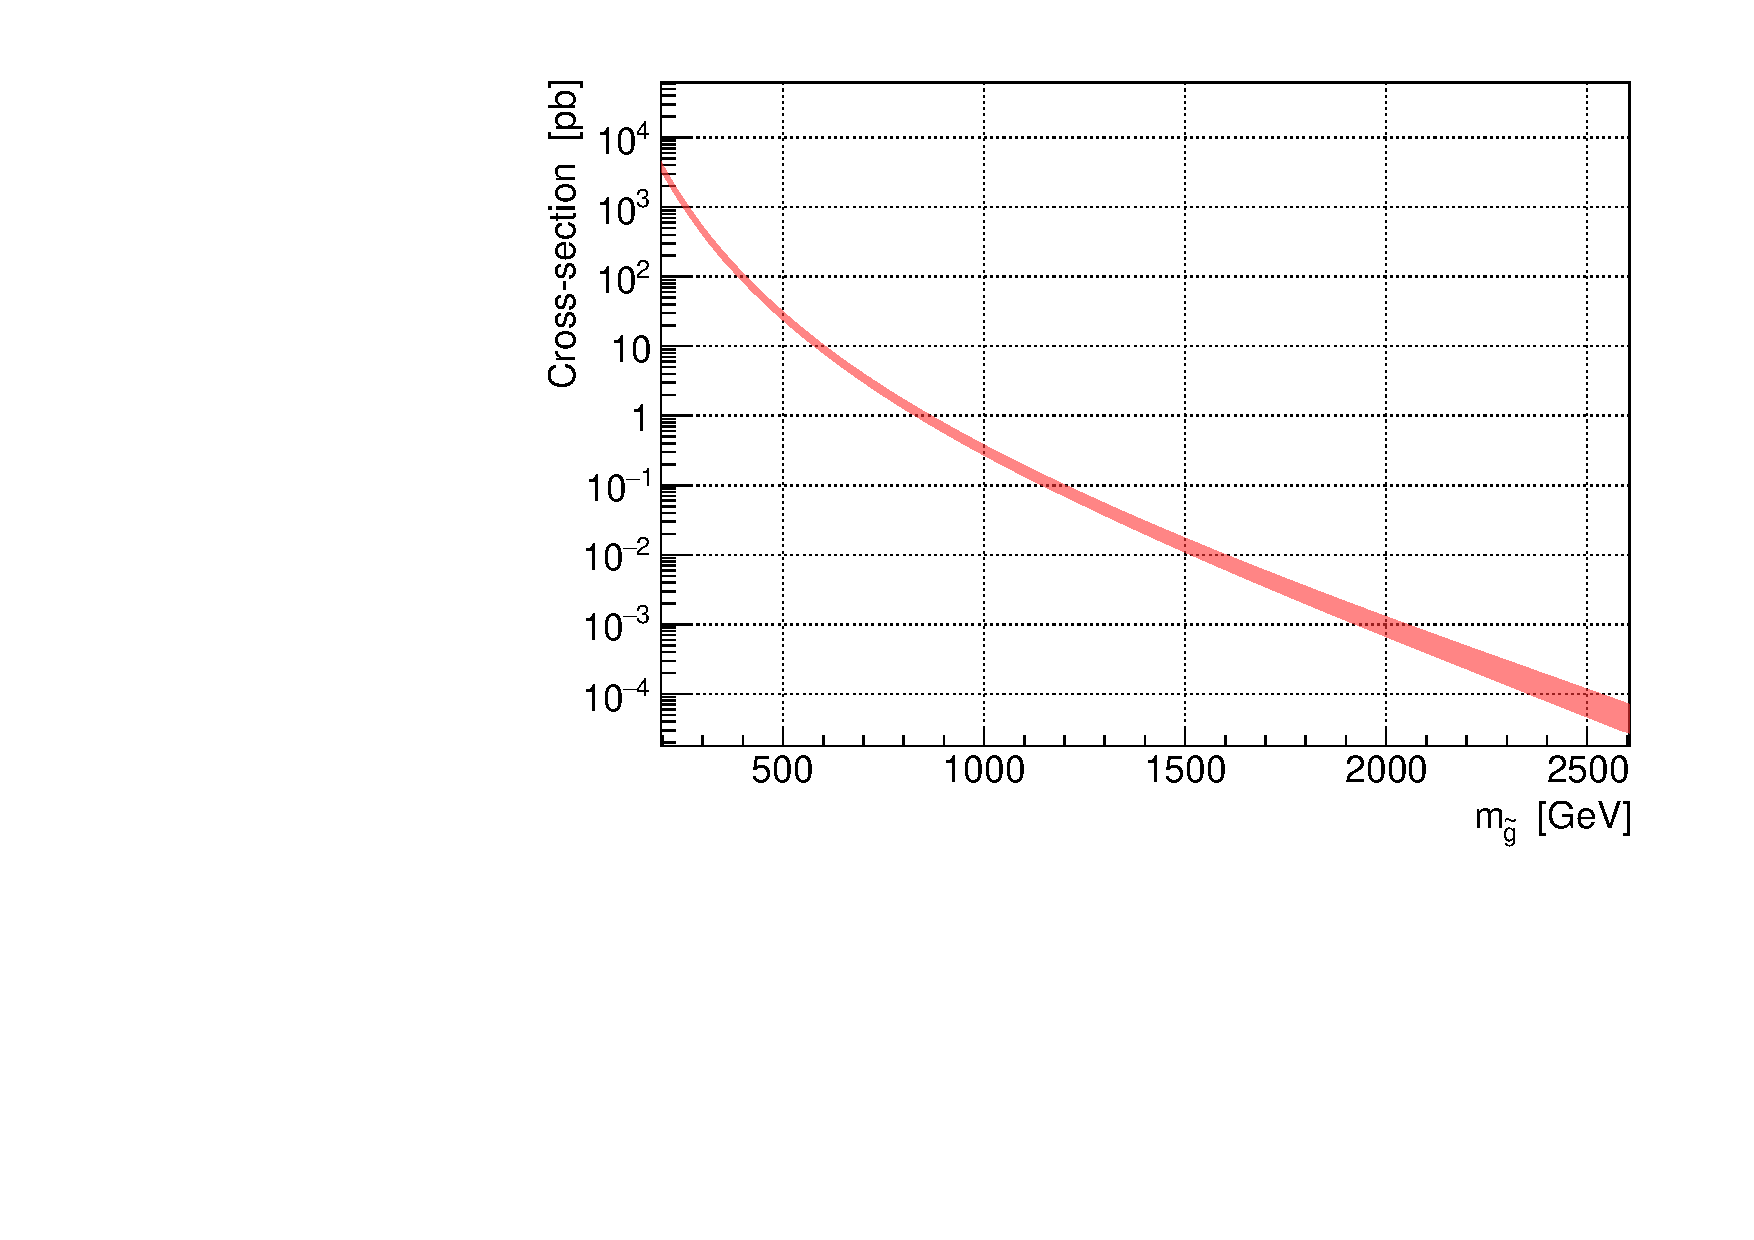
\includegraphics[width=140mm]{figures/Samples/xsec_GG/xsec_GG.pdf}
    \captionof{figure}{Cross-section for gluino pair production. Calculation is performed at NNLO+NNLL accuracy.}
    \label{fig::Samples::xsec_GG}
  \end{center}
\end{figure}
%-------------------------------     


\noindent Further caveats particular to each process are stated as below.
% ($W$/$Z$+jets)~\cite{ATL-PHYS-PUB-2016-003}

\paragraph{$W/Z$+jets} 
%Events containing $W$ or $Z$ bosons with associated jets are simulated using the \sherpa2.2.1 generator~\cite{Gleisberg:2008ta}
The matrix elements are calculated using the \sherpa2.2.1 generator~\cite{Gleisberg:2008ta} up to two partons at NLO and four partons at LO\@ using the Comix~\cite{Gleisberg:2008fv} and OpenLoops~\cite{Cascioli:2011va} generators. 
They are merged with the \sherpa2.2.1 parton shower~\cite{Schumann:2007mg} with massive $b$ and $c$ quarks using the ME+PS@NLO prescription~\cite{Hoeche:2012yf}.
The CKKW scheme is used for ME/PS matching with matching scale set to $30\gev$.


% ttbar, 1top  $Wt$ and $s$-channel~\cite{ATL-PHYS-PUB-2016-004},
\paragraph{Tops: $\ttbar$/single-top}
The EvtGen v1.2.0 program is used to describe the properties of the bottom and charm hadron decays in the \ttbar\ and the single-top-quark samples. 
The $h_{\rm damp}$ parameter, which controls the \pt\ of the first additional emission beyond the Born configuration, is set to the mass of the top-quark. 
The main effect of this is to regulate the high \pt\ emission against which the \ttbar\ system recoils. The top-quark mass is set to $172.5 \gev$ for all the samples. 

\paragraph{Di-bosons: WW/WZ/ZZ}
The fully-leptonic processes are simulated with five final states ($\ell\ell\ell\ell$, $\ell\ell\ell\nu$, $\ell\ell\nu\nu$, $\ell\nu\nu\nu$, $\nu\nu\nu\nu$). The intermediated states are not specified therefore the contribution from Drell-Yan-like off-shell diboson and the interference between different diboson processes (e.g. $WW\ra\ell\ell\nu\nu$ and $WZ\ra\ell\ell\nu\nu$) are taken into account. The semi-leptonic diboson processes are simulated with designated intermediated boson states namely $W$ or $Z$.
%The processes are calculated for up to one parton (for $ZZ$) or no additional partons (for $WW, WZ$) at NLO and up to three partons at LO using the Comix and OpenLoops matrix-element generators.
The cross-section is calculated at NLO order for each diboson channel $WW,WZ,ZZ$ ~ to which the samples are normalized to.


%For the $t\bar{t}+W/Z/WW$ processes~\cite{ATL-PHYS-PUB-2016-005}
\paragraph{${\bf \ttbar+W/Z/WW}$}
All processes are simulated by \mgmc 2.2.3 at LO interfaced to the \pythia 8.186 parton shower model, 
with up to two ($t\bar{t}+W$), one ($t\bar{t}+Z$) or no ($t\bar{t}+WW$) extra partons included in the matrix element. 
The EvtGen v1.2.0 program~\cite{EvtGen} is used to describe the properties of the bottom and charm hadron decays. 
The ATLAS shower and underlying-event tune A14 is used together with the NNPDF2.3~LO PDF set. 
The events are normalized to their NLO cross-sections~.


\paragraph{SUSY signals} \label{sec::Samples::SUSY}
The EvtGen v1.2.0 program~\cite{EvtGen} is used to correct the description of the bottom and charm hadron decays. 
Decay of EW gauginos are done in \pythia , based on phase space with no consideration of the spin.
The CKKW-L matching scheme~\cite{CKKW} is applied for the matching of the matrix element and the parton shower, with the correspoding scale parameter set to 1/4 of the gluino mass. 
The cross-section uncertainty are taken from an envelope of cross-section predictions using different PDF sets and factorization and renormalisation scales, as described in Ref.~\cite{Borschensky:2014cia}, considering only the four light-flavor left-handed squarks ($\tilde{u}_L$, $\tilde{d}_L$, $\tilde{s}_L$, and $\tilde{c}_L$). Fig. \ref{fig::Samples::xsec_GG} shows the calculated cross-section and the associated error. \\

Model parameters irrelevant to SUSY masses are fixed to arbitrary reasonable values, 
since here we assume they do not change the kinematics as disscussed in Sec. \ref{sec::Introcution}.
The mixing parameters are set so that LSP and NLSP are bino- and wino-like. \\



\subsubsection{Pileup simulation}
All simulated events are generated with a varying number of minimum-bias interactions overlaid on the hard-scattering event to model the multiple proton-proton interactions in the same and the nearby crossing crossings.
The minimum-bias interactions are simulated with the soft QCD processes of \pythia8.186 using the A2 tune \cite{ATLAS:2012uec} and the MSTW2008LO PDF set~\cite{Martin:2009iq}. 
Corrections are applied to the samples to account for differences between data and simulation for trigger, identification and reconstruction efficiencies. \\



\subsubsection{Detector Simulation and Emulation}
The detector response to generated particles is simulated by a full ATLAS detector simulation model \cite{ATLASFullSimu:2010wqa} based on \textsc{Geant4}~\cite{Agostinelli:2002hh}, for the background samples. \\

The ATLAS fast simulation ~\cite{atlfast} is used for signal models marked as $\checkmark$ in Tab. \ref{tab::Introduction::modelsBV}-\ref{tab::Introduction::models3B} in Sec. \ref{sec::Introduction::targetModels}, as the economical alternative. This is based on a parametrization of the performance of the electromagnetic and hadronic calorimeters and on \textsc{Geant4} elsewhere. The difference between the full simulation is found to be marginal after examining a number of reference signal points.
The subsequent procedures are identical to what is processed for the data sample: particle reconstruction and identifications, as described in Sec. \\

For the signal models with no $\checkmark$ in Tab. \ref{tab::Introduction::modelsBV}-\ref{tab::Introduction::models3B}, no detector simulation nor reconstruction is performed. Instead the effect is emulated by smearing the energy of truth-level particles and clustered jets, based on the resolution parametrized using the full simulated samples. The object identification is emulated by randomly accepting the candidates at the rate of the parametrized efficiency. The modeling is extensively tested by comparing the kinematic distributions with the fast simulated samples. The discrepancy is found sufficiently small, staying within 5$\%$ in general and never exceed $10\%$. \\

% benchmark models
% non-benchmark models -> no detector simulation, use emulation


\subsection{Design of SUSY Signal Grid for Interpretation} 
Obtained exlusion limits are presented in form of contours in a 2-dimensional plane, usually in terms of SUSY masses. This is done by generating a set of signal samples with various SUSY masses covering the whole plane with discrete steps, referred as a signal grid, and the results of the hypothetical test for the points are interpolated, providing continuous limit in the end. \\

For limits on the direct decay models, $\mG$ and $\mLSP$ are chosen as x and y-axis respectively to represent (referred as ``\dire'' grid). The cases with 1-step decay models is a bit tricky, since they involve the third mass; the intermediate EW-gaugino $\chaone$ or $\neutwo$. The full 3-dimensional presentation is not realistic from computational cost of view, due to the enormously increased number of grid points to cover the whole grid. Therefore, a couple of sensible 2D-slices are made that sufficiently capture the essence of the 3D-grid. ``\xhalf'' is the grid with the intermediate EW-gaugino mass is set to midmost between gluino and the LSP, while $x$ is defined as a parameter representing the relative mass splitting:
\begin{align}
  x := \dmcn/\dmg, \,\,\,\,\,\,\, x \in [0,1]. \nn
\end{align}
The \varx grid is then designed to complement the hole in high or low $x$, where the LSP mass is fixed to $60\gev$ and the gluino mass and the intermediate EW-gaugino mass are set free. There are two additional grids \DMtw and \DMth in which the intermediate EW-gaugino an the LSP are compressed ($\dmcn=20, \, 30\gev$ respectively), respecting the dark matter relic constraint in discussed in Sec. \ref{sec::Introduction::DMconstraint}. Note that these DM grids are not considered in models with $\neutwo$ decaying to higgs, since higgs is too far off-shell thus $\neutwo$ never almost decays via higgs in the situation. \\
To summarize, four types of signal grid are designed in the analysis, as shown in Tab. \ref{tab::Samples::signalGridDef}. 


%\tabsmall{ c | c c c c}
\tab{ c | c c c c}
{
\hline
Grid name   & x-axis   & y-axis         & Slicing                & Note\\
\hline
\hline
\dire       & $\mG$   & $\mLSP$         &  -                     & - \\
\hline
\hline
\xhalf      &  $\mG$  & $\mLSP$         &  $\dmg = \dmcn$        & - \\
\varx       &  $\mG$  & $\dmcn / \dmg$  &  $\mLSP=60\gev$        & - \\
\DMtw,\DMth &  $\mG$  & $\mLSP$         &  $\dmcn=20,30\gev$     & For models without \\
            &         &                 &                        & $h$-mediated $\tilde{\chi}_2^0$ decays. \\
\hline
}
{List of signal grids used for limit setting. \dire is for the direct decay model, and the others are for the 1-step decay models. The latter is four-fold: \xhalf, a grid with EW gaugino mass fixed to the middle of gluino and LSP; \varx, in which LSP mass is fixed to 60$\gev$; \DMtw and \DMth are grids with $\dmcn=20,30\gev$ which are considered only in models without $\neutwo$ decay into higgs. }
{tab::Samples::signalGridDef}



